\section{\todo{Going Further}}

% --------------------------------
%          High Ranges
% --------------------------------
\subsection{\review{High Ranges}}

% --------------------------------
%          High Ranges
\subsubsection{\review{Limitations}}

So far, the momentum offset ranges of the 2024 measurements have been restricted in order to allow a 
comparison with the shorter ranges measurements made in 2022. The non-linearity of the chromaticity 
and its higher orders become very noticeable once these large ranges are reached.
\Cref{fig:high_orders:chroma_nominal_correction_full_range} shows an example of such measurement for 
Beam 2, made with the nominal corrections, highlighting the difference between two momentum offset
ranges.

\begin{figure}[!htb]
    \begin{subfigure}{0.49\textwidth}
        \centering
        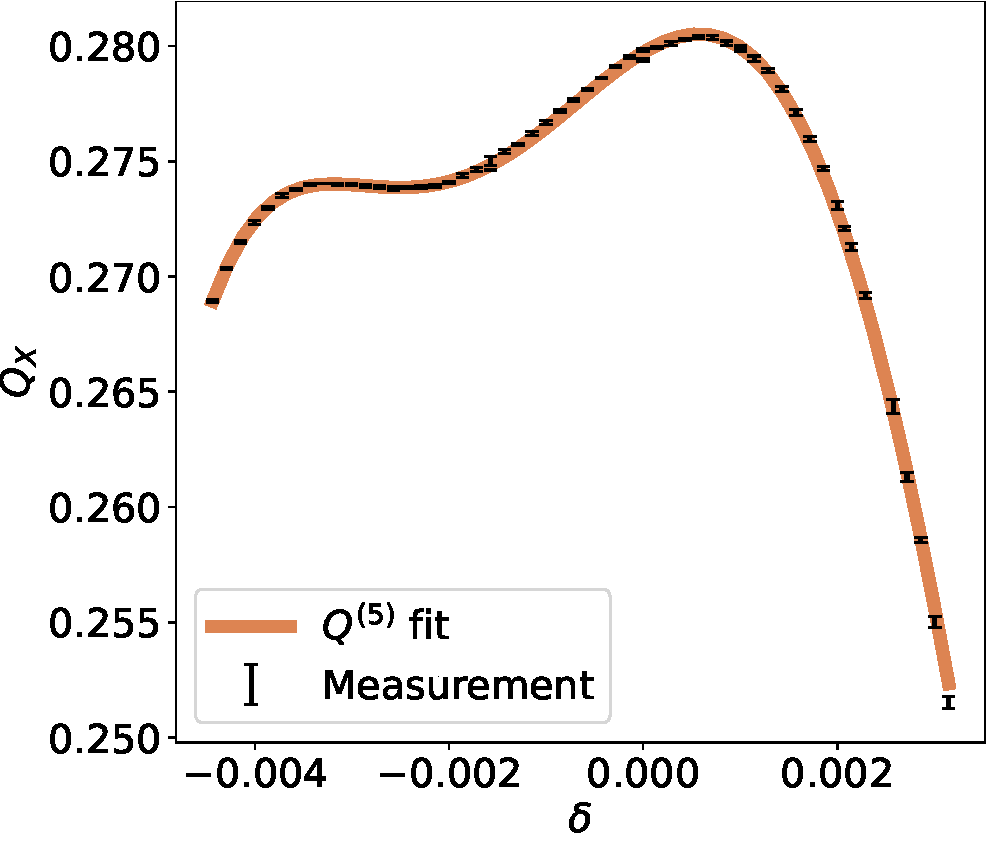
\includegraphics[width=\textwidth]{./images/chromaticity_further/q5_range/Beam2_Qx_full_but_not_quite.pdf}
        \caption{$Q_x$ Beam 2 High Range}
    \end{subfigure}
    \hfill
    \begin{subfigure}{0.49\textwidth}
        \centering
        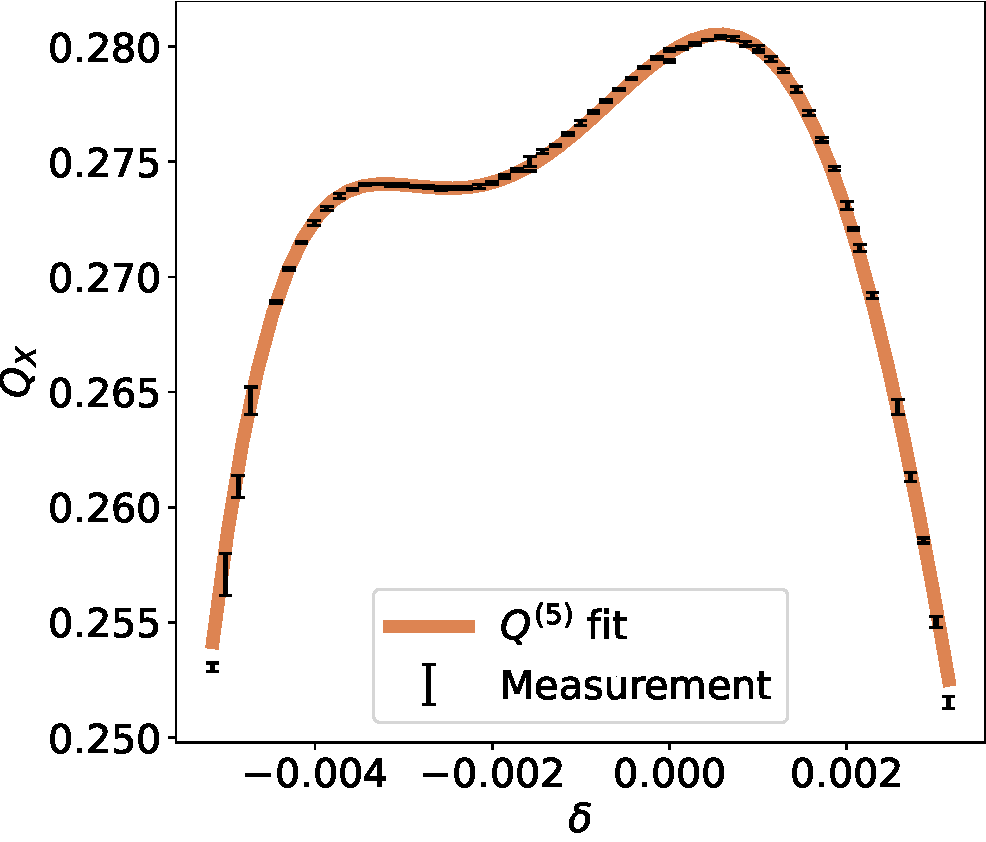
\includegraphics[width=\textwidth]{./images/chromaticity_further/q5_range/Beam2_Qx_full.pdf}
        \caption{$Q_y$ Beam 2 Full Range}
    \end{subfigure}
    %
    \caption{Third Beam 2 measurement of \cref{table:high_orders:dpp_ranges} with nominal
    corrections. A very large momentum offset range clearly highlights the non-linearity of the
    chromaticity function.}
    \label{fig:high_orders:chroma_nominal_correction_full_range}
\end{figure}

\begin{table}[!htb]
    \centering
    \begin{tabular}{lcccc}
      \toprule
      Plane & $Q^{(2)} [\times 10^{3}]$ & $Q^{(3)} [\times 10^{6}]$ & $Q^{(4)} [\times 10^{9}]$ & $Q^{(5)} [\times 10^{12}]$ \\
      \midrule
      X &&&& \\  
      \hspace{2mm}Rest. Range &$-2.93 \pm 0.05$ & $-4.40 \pm 0.08$ & $-0.53 \pm 0.08$ & $ 1.66 \pm 0.16$ \\
      \hspace{2mm}High Range  &$-2.99 \pm 0.05$ & $-4.71 \pm 0.03$ & $-0.42 \pm 0.07$ & $ 2.23 \pm 0.07$ \\
      \hspace{2mm}Full Range  &$-3.05 \pm 0.05$ & $-4.75 \pm 0.03$ & $-0.33 \pm 0.07$ & $ 2.34 \pm 0.06$ \\
      Y &&&& \\  
      \hspace{2mm}Rest. Range &$ 0.89 \pm 0.02$ & $ 2.05 \pm 0.03$ & $ 0.32 \pm 0.03$ & $-0.73 \pm 0.06$ \\
      \hspace{2mm}High Range  &$ 0.87 \pm 0.02$ & $ 2.07 \pm 0.02$ & $ 0.36 \pm 0.03$ & $-0.77 \pm 0.03$ \\
      \hspace{2mm}Full Range  &$ 0.70 \pm 0.04$ & $ 1.83 \pm 0.03$ & $ 0.64 \pm 0.06$ & $-0.32 \pm 0.05$ \\
      \bottomrule
    \end{tabular}
    \caption{Variance of the chromaticity values depending on the considered momentum offset range.
    All ranges have an upper bound of $3.2\times10^{-3}$. The lower bounds are, in order of
    appearance: $-3.5$, $-4.5$, $-5.2$.}
    \label{tab:high_orders:further:chroma_different_ranges}
  \end{table}

\Cref{tab:high_orders:further:chroma_different_ranges} shows the obtained chromaticity values for
varying ranges. From this table, it can be noted that increasing the range mainly
changes the estimate for $Q^{(5)}_x$.
Measurements over such a wide range are not yet fully understood, as other non-linear effects can
induce a detuning. For example, transverse impedances leads to a defocusing effect whose magnitude
increases with the orbit offset~\cite{antipov_single-collimator_2018,kurtulus_lhc_2022}.
Some other performed measurements with wide ranges in 2024 could not be fitted with a chromaticity
function, despite including higher orders. It is deemed that restricting the ranges is beneficial to
the fit estimates, until further investigation of these effects.



% --------------------------------
%       Even Higher Orders?
\subsubsection{\review{Higher Orders}}

The fifth measurement in \cref{table:high_orders:dpp_ranges} covered a range of $[-4.0 \cdot
10^{-3}, 4.5 \cdot 10^{-3}]$, which is among the widest ever measured. It is clear from
\cref{fig:high_orders:chroma_after_correction_full_range} that a chromaticity function including the
sixth order provides a better fit to the data. However, no additional observations were made for
this order, and considering the previously mentioned limitations, this measurement may not be
entirely robust. Further studies could address these limitations to more accurately characterize the
decahexapolar fields of the LHC at injection energy.

\begin{figure}[!htb]
    \begin{subfigure}{0.49\textwidth}
        \centering
        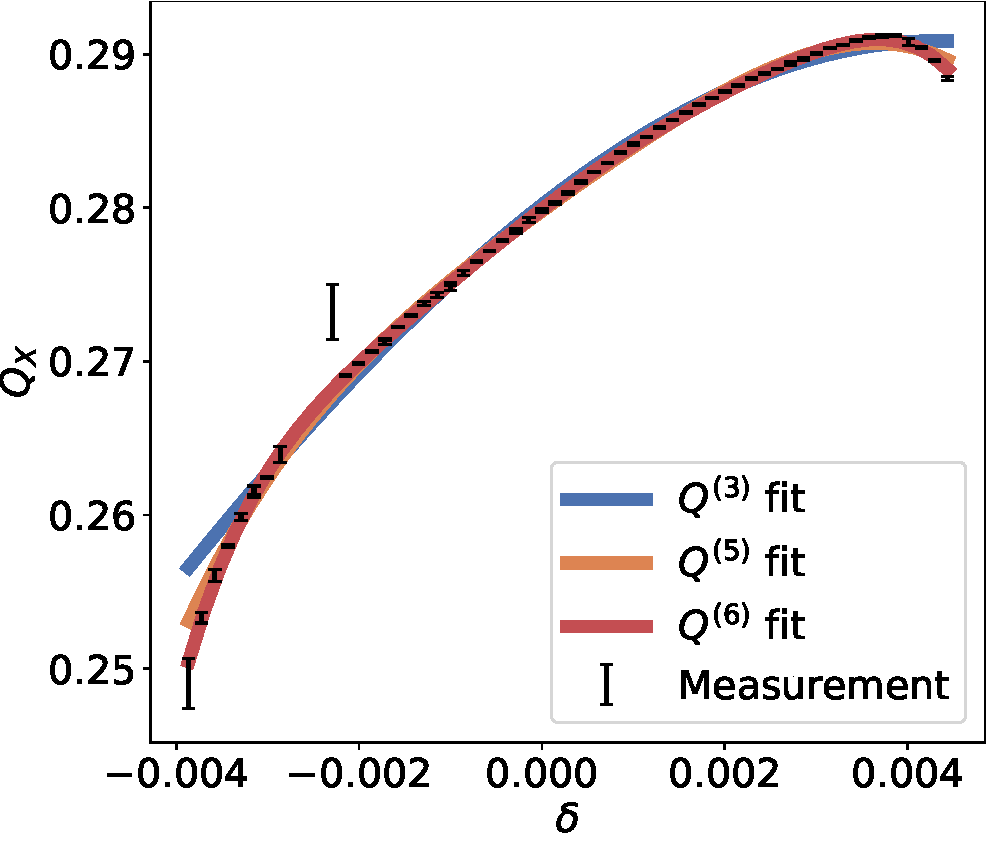
\includegraphics[width=\textwidth]{./images/chromaticity_further/q6/Beam1_Qx.pdf}
        \caption{$Q_x$ Beam 1}
    \end{subfigure}
    \hfill
    \begin{subfigure}{0.49\textwidth}
        \centering
        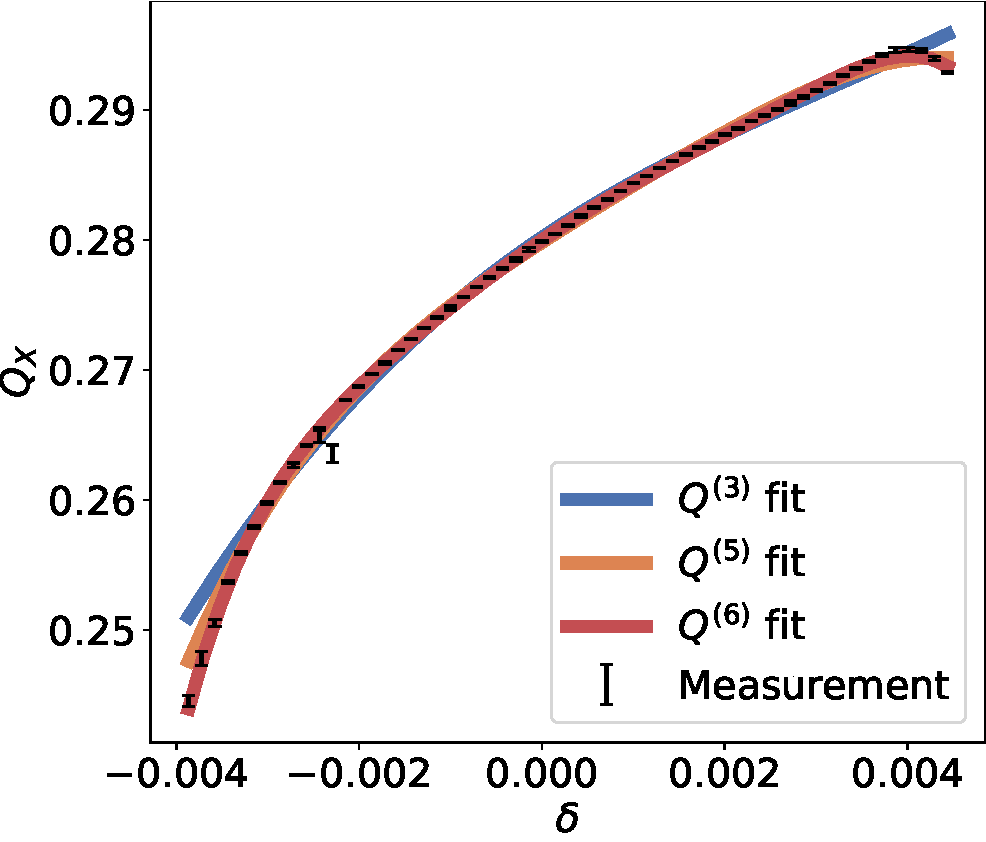
\includegraphics[width=\textwidth]{./images/chromaticity_further/q6/Beam2_Qx.pdf}
        \caption{$Q_x$ Beam 2}
    \end{subfigure}
    %
    \caption{Fifth measurement of \cref{table:high_orders:dpp_ranges} with $Q''$ and $Q'''$
    corrections. A possible sixth chromaticity order can be seen.}
    \label{fig:high_orders:chroma_after_correction_full_range}
\end{figure}

